\pdfbookmark[0]{Remerciements}{Remerciements}
\chapter*{Remerciements}
\label{sec:remerciements}
\vspace*{-10mm}

\cleanchapterquote{
%
Just do it.\\
Make your dreams come true.\\
Nothing is impossible.\\
Yes you can.
%
}{Shia \textsc{LaBeouf}}{}

C'est marrant, au début de ma thèse, le moment où j'allais rédiger cette page
des remerciements me paraissait tellement loin. Et maintenant, j'en suis à cette
étape. C'est marrant.

Et si j'en suis à écrire ces mots, c'est en grande partie grâce à David
\textsc{Coeurjolly} et Jacques-Olivier \textsc{Lachaud}, qui m'ont fait
confiance et m'ont soutenu, surtout dans les moments de doute, tout au long de
cette thèse. C'était un vrai plaisir de travailler avec vous, de discuter avec
vous. J'ai énormément appris grâce à vous et je vous en suis très reconnaissant.

Je remercie les membres de mon jury, Nicolas \textsc{Passat}, Pierre
\textsc{Alliez}, Éric \textsc{Andrès}, Yan \textsc{Gérard}, Simon
\textsc{Masnou} pour voir répondu sans hésitation favorablement à l'évaluation
de mon travail et pour leurs retours.

L'ambiance au travail est primordiale. À ce titre, je remercie \emph{énormément}
les membres du LIRIS-1\footnote{Élu meilleur bureau de doctorants trois années
consécutives par un panel non représentatif.} -- Elsa, Abdoulaye, François,
Grégoire, Jean-David, Gérémy, Matthieu --. Je ne pourrais pas énumérer la liste
des choses qui se sont produites dans ce bureau lors de moments de « craquages »
tellement la liste est longue (voir la \RefFigure{fig:jerem-in-the-truck}),
allant des combats de NERF aux blind tests d'OST de jeux vidéos, en passant par
les sessions d'EuroTruck Simulator 2 avec Oculus Rift et volant. Je ne pense pas
qu'on puisse faire de meilleure ambiance au travail que celle-ci. Merci.
%
\begin{figure}[ht]{
  \begin{center}
    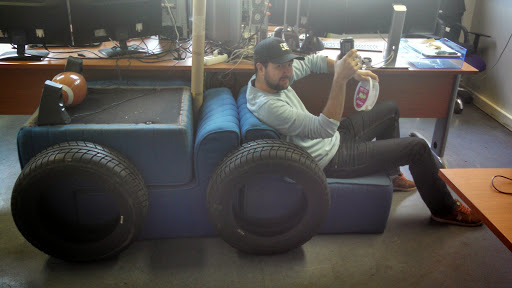
\includegraphics[width=8cm]{images/misc/JeremInTheTruck}
  \end{center}
  \caption{Reproduction à l'échelle $1:10$ d'un camion avec le mobilier à disposition.\label{fig:jerem-in-the-truck}}}
\end{figure}

Merci également aux « amis du LIRIS-1 », contribuant à l'esprit LIRIS-1 --
Hélène, Karolina, Lucille, Marie-Neige, Rubiela, David, Joseph --. Ces (\emph{un
peu moins de}) quatre années de thèse ont été un vrai plaisir en votre
compagnie. Parce qu'il n'y a pas que le travail dans la vie, ces années de
thèses ont été sublimés (tel un gâteau dans Top Chef) grâce à vous par quelques
sorties « extra-scolaires » : journées au ski, laser game, course à pied, VTT et
j'en passe. C'était vraiment cool et parfois ça fait du bien de se vider la
tête.

Je ne remercie pas la SNCF, pour avoir rendu mes trajets à Chambéry de
véritables calvaires à coups de « Perte d'adhérence sur les rails » ou de «
Raté d'ouverture d'un passage à niveau ».

Un grand merci aux secrétaires du LIRIS et du LAMA, surtout à Sylvie qui m'a
débloqué pas mal de situations dont un fameux appel, un lundi matin : «
Euh ... je crois que j'ai raté mon avion. Je fais quoi ? ».

Merci également à mes collègues au sein des équipes M2DisCo et LIMD, et plus
largement au LIRIS et au LAMA, ainsi que de l'ANR digitalSnow pour ces
discussions riches autour de domaines variés.

J'ai une pensée pour Yoann \textsc{Pigné} -- à l'époque doctorant à l'Université
du Havre lors de ma première année de Licence -- qui, sans le savoir, m'a donné
envie de faire une thèse.

Une pensée également au club des \emph{gentlemen}, « Les Barons », -- Mierre,
Dhomas, Grançois, TFC -- dont les nombreuses soirées « Rétro-bièring » et les
discussions autour des jeux vidéos, de l'informatique ou des sciences en général
ont été une source inépuisable d'échange de connaissance. Je ramène un jeu NES
de ma collection pour la prochaine soirée.

Je suis extrêmement redevable envers mes « conseillers personnels » -- Dav,
\barre{Léa} Zouille, JD, L0ur5, Sandrine -- qui ont su m'aiguiller lors des
moments de doute.

Un petit mot aussi à Marion, Thomas, (Hélène ?), doctorants avec lesquels je
partage au moins un encadrant. Je vous souhaite bon courage pour la suite de
votre thèse. Vous verrez, la soutenance arrive vite !

Enfin, et non des moindre, je voudrais remercier mes parents et mes soeurs qui
n'ont eu de cesse de me soutenir, même s'ils ne comprenaient pas vraiment ce que
je faisais. Je remercie bien évidemment Audrey pour m'avoir épaulé chaque jour.

Avant de vous laisser lire le contenu plus \emph{scientifique} (ou bien me
rédiger un mail d'insulte parce que je vous ai oublié dans ces
remerciements\footnote{Si c'est le cas, les sources de ma thèse sont disponibles
sur GitHub : \url{https://github.com/jlevallois/PhD-Thesis}, faites un
pull-request pour vous rajouter.}), je voudrais revenir sur les citations en
début de chapitre. Ne cherchez pas de cohérence avec le contenu des chapitres,
celles-ci ont été choisies car elles représentent quelque chose qui a été
important pour moi (un livre, un film, une série). C'est pour moi, en quelque
sorte, un moyen de remercier l'auteur.
